\section{System Identification}
\label{sec:sysid}

%% FIG: MODEL VS. WEIGHT OF L1 PENALTY (LASSO)
\begin{figure}
    \centering
    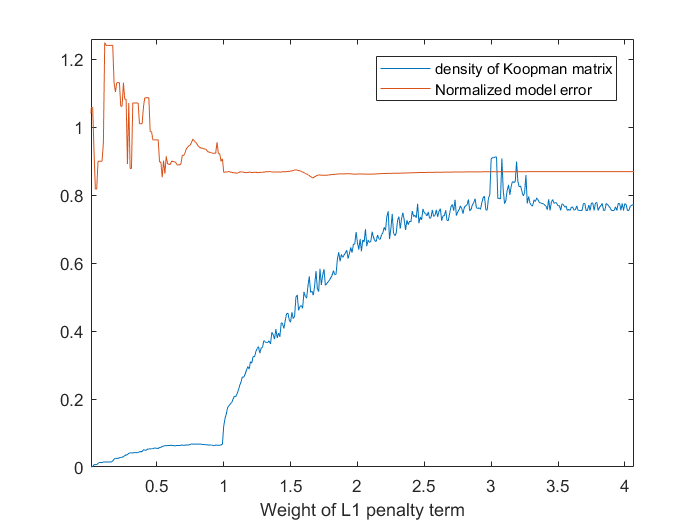
\includegraphics[width=\linewidth]{figures/lasso_placeholder.png}
    \caption{As the weight of the L1 penalty term increases, the Koopman operator matrix becomes more dense, and the model error decreases then levels off. This shows that there is a much sparser representation of the Koopman operator than the least-squares solution that generates a model of nearly identical accuracy.}
    \label{fig:lasso}
\end{figure}


%% Overview of this section
Any finite-dimensional nonlinear dynamical system has an equivalent infinite-dimensional linear representation in the space of real-valued functions of the system's state \cite{}.
In this function space, the (linear) Koopman Operator describes the flow of functions along trajectories of the system.
% The dual of the Koopman operator, the Perron-Frobenius operator, describes the dynamics of the system...
While it is not possible to fully represent the infinite-dimensional Koopman operator, it is possible to represent its projection onto a finite-dimensional subspace.

%% Overview of the Koopman operator and how it represents dynamical systems
\subsection{Koopman Representation of Dynamical Systems}

%% System representation in state space
Consider a dynamical system
\begin{align}
    \dot{x} &= F (x)    \label{eq:nlsys}
\end{align}
where $x \in \Real^n$ is the state of the system and ${F}$ is continuously differentiable in $x$.
Denote by $\phi(t,x_0)$ the solution to \eqref{eq:nlsys} at time $t$ when beginning with the initial condition $x_0$ at time $0$.
For simplicity, we denote this map, which is referred to as the \emph{flow map}, by $\phi^t (x_0)$ instead of $\phi (t, x_0)$.

%% System representation in the space of observables
The system can be lifted to an infinite dimensional function space $\mathcal{F} = L^2(X, \Real)$ where $X \subset \Real^n$ is a compact subset and $L^2(X , \Real)$ is the space of square integrable real-valued functions with domain $X$.
Elements of $\mathcal{F}$ are called \emph{observables}.
In $\mathcal{F}$, the flow of the system is characterized by the set %semigroup 
of Koopman operators 
$U^t : \mathcal{F} \to \mathcal{F}$, for each $t \geq 0$,
which describes the evolution of the observables ${f \in \mathcal{F}}$ along the trajectories of the system according to the following definition:
\begin{align}
    U^t f = f \circ \phi^t      
    % && \forall f \in \F, t \geq 0
    \label{eq:koopman}
\end{align}
As desired, $U^t$ is a linear operator even if the system \eqref{eq:nlsys} is nonlinear, since for $f_1, f_2 \in \mathcal{F}$ and $\lambda_1, \lambda_2 \in \Real$
\begin{align}
    \begin{split}
    U^t (\lambda_1 f_1 + \lambda_2 f_2) &= \lambda_1 f_1 \circ \phi^t + \lambda_2 f_2 \circ \phi^t \\
    &= \lambda_1 U^t f_1 + \lambda_2 U^t f_2.
    \end{split}
\end{align}
Thus the Koopman operator provides a linear representation of the flow of a nonlinear system in the infinite-dimensional space of observables (see Fig. \ref{fig:overview}) \cite{budivsic2012applied}.


%% Koopman-based system identification (consult ICRA paper)
\subsection{Identification of Koopman Operator}

Since the Koopman operator is an infinite-dimensional object, it cannot be represented by a finite-dimensional matrix. 
Therefore, we settle for the projection of the Koopman operator onto a finite-dimensional subspace.
Using the system identification method originally presented in \cite{mauroy2016linear} and \cite{mauroy2017koopman}, we identify a finite-dimensional approximation of the Koopman operator via linear regression performed on observed data.

Define ${\bar{\mathcal{F}} \subset \mathcal{F}}$ to be the subspace of $\mathcal{F}$ spanned by $N$ linearly independent basis functions $\{ \psi_k \}_{k=1}^N$.
Any observable $\bar{f} \in \bar{\mathcal{F}}$ can be expressed as a linear combination of elements of these basis functions
\begin{align}
    \bar{f} &= \alpha_1 \psi_1 + \cdots + \alpha_N \psi_N
\end{align}
where each $\alpha_i \in \Real$.
For notation, we introduce the vector of coefficients ${\alpha = [ \alpha_1 \,  \cdots \, \alpha_N ]^T}$ and the \emph{lifting function} $\psi : \Real^n \to \Real^N$ defined as:
\begin{align}
    \psi(x) &:= \begin{bmatrix} \psi_1 (x) & \cdots & \psi_N (x) \end{bmatrix}^T.
    \label{eq:lift}
\end{align}
Then, $\bar{f} \in \bar{\mathcal{F}}$ can be expressed concisely as
\begin{align}
    \bar{f} &= \alpha^T \psi
    \label{eq:fvec}
\end{align}
Via \ref{eq:fvec}, $\alpha$ provides a vector representation for $\bar{f} \in \bar{\mathcal{F}}$.

Given this vector representation for observables, a finite-dimensional approximation of the Koopman Operator can be represented by a matrix.
We denote by $\bar{U}^t \in \Real^{N \times N}$ the approximation of the Koopman Operator in $\bar{\mathcal{F}}$, which operates on observabels via matrix multiplication:
\begin{align}
    \bar{U}^t \alpha = \beta
\end{align}
where $\alpha , \beta$ are each vector representations of observables in $\bar{\mathcal{F}}$.
%% Pulled straight from ICRA paper below this line
Our goal is to find a $\bar{U}^t$ that describes the action of the infinite dimensional Koopman operator $U^t$ as accurately as possible in the $L^2$-norm sense on the finite dimensional subspace $\bar{\mathcal{F}}$  of all observables.
Therefore, to perfectly mimic the action of $U^t$ acting on an observable in $\bar{\mathcal{F}} \subset \mathcal{F}$, the following should be true
\begin{align}
    ( \bar{U}^t {\alpha} )^T {\psi}(x) &=
    {\alpha}^T {\psi} \left( \phi^t(x) \right).
    \label{eq:UbarEq}
\end{align}
Since this is a linear equation, it follows that for a given ${x \in \Real^n}$, solving \eqref{eq:UbarEq} for $\bar{U}^t$ yields the best approximation of $U^t$ on $\bar{\mathcal{F}}$ in the $L^2$-norm sense:
\begin{align}
    \bar{U}^t = \left( {\psi}(x)^T \right)^\dagger {\psi}( \phi^t(x) )^T
    \label{eq:Uapprox}
\end{align}
where superscript $\dagger$ denotes the least-squares pseudoinverse.

%% How this is done on our system
To approximate the Koopman operator from a set of experimental data, we take $K+1$ discrete state measurements with sampling period $T_s$. We separate the data into a set of $K$ so-called ``snapshot pairs'' of the form ${ \{ x_k , y_k \} \in \Real^{n \times 2} }$ where
\begin{align}
    y_{k} &= \phi^{T_s} (x_k) + \sigma_k
\end{align}
and $\sigma_k$ denotes measurement noise.
% For our basis of $\bar{\mathcal{F}}$, we choose the basis of monomials of $x$ with total degree less than or equal to $w$, which implies ${N=(n+m+w)!/\left((n+m)!w!\right)}$ \cite[Section III]{mauroy2016linear}. 
We then lift all of the snapshot pairs according to \eqref{eq:lift} and compile them into the following ${K \times N}$ matrices:
\begin{align}
    &\Psi_x = \begin{bmatrix} {\psi}(x_1)^T \\ \vdots \\  {\psi}(x_K)^T \end{bmatrix}
    &&\Psi_y = \begin{bmatrix} {\psi}(y_1)^T \\ \vdots \\  {\psi}(y_K)^T \end{bmatrix}
\end{align}
$\bar{U}^{T_s}$ is chosen so that it yields the least-squares best fit to all of the observed data, which, following from \eqref{eq:Uapprox}, is given by 
\begin{align}
    \bar{U}^{T_s} &:= \Psi_x^\dagger \Psi_y.
\end{align}

%% The Koopman MPC problem (consult Mezic paper)
\subsection{Model Predictive Control}